\chapter{Background}
\label{ch:Chapter2}

This chapter provides background that is required for understanding the mechanisms of our technique. We provide a short summary of conventional control theory systems followed by DNN based systems, and the different roles of people in the work. We finally end the chapter with a formal definition of our problem statement. 



%We consider a closed-loop system as shown in Figure 2, with sensors as the inputs to the DNN and the actuators that take the output from the DNN based controllers. We describe the model for CPS, followed by the DNN controller model, attack model formalism and the problem statement.

%\aarti{Should the diagram be more descriptive with DNNs in the middle?}
\iffalse
\begin{figure}
	\centering
	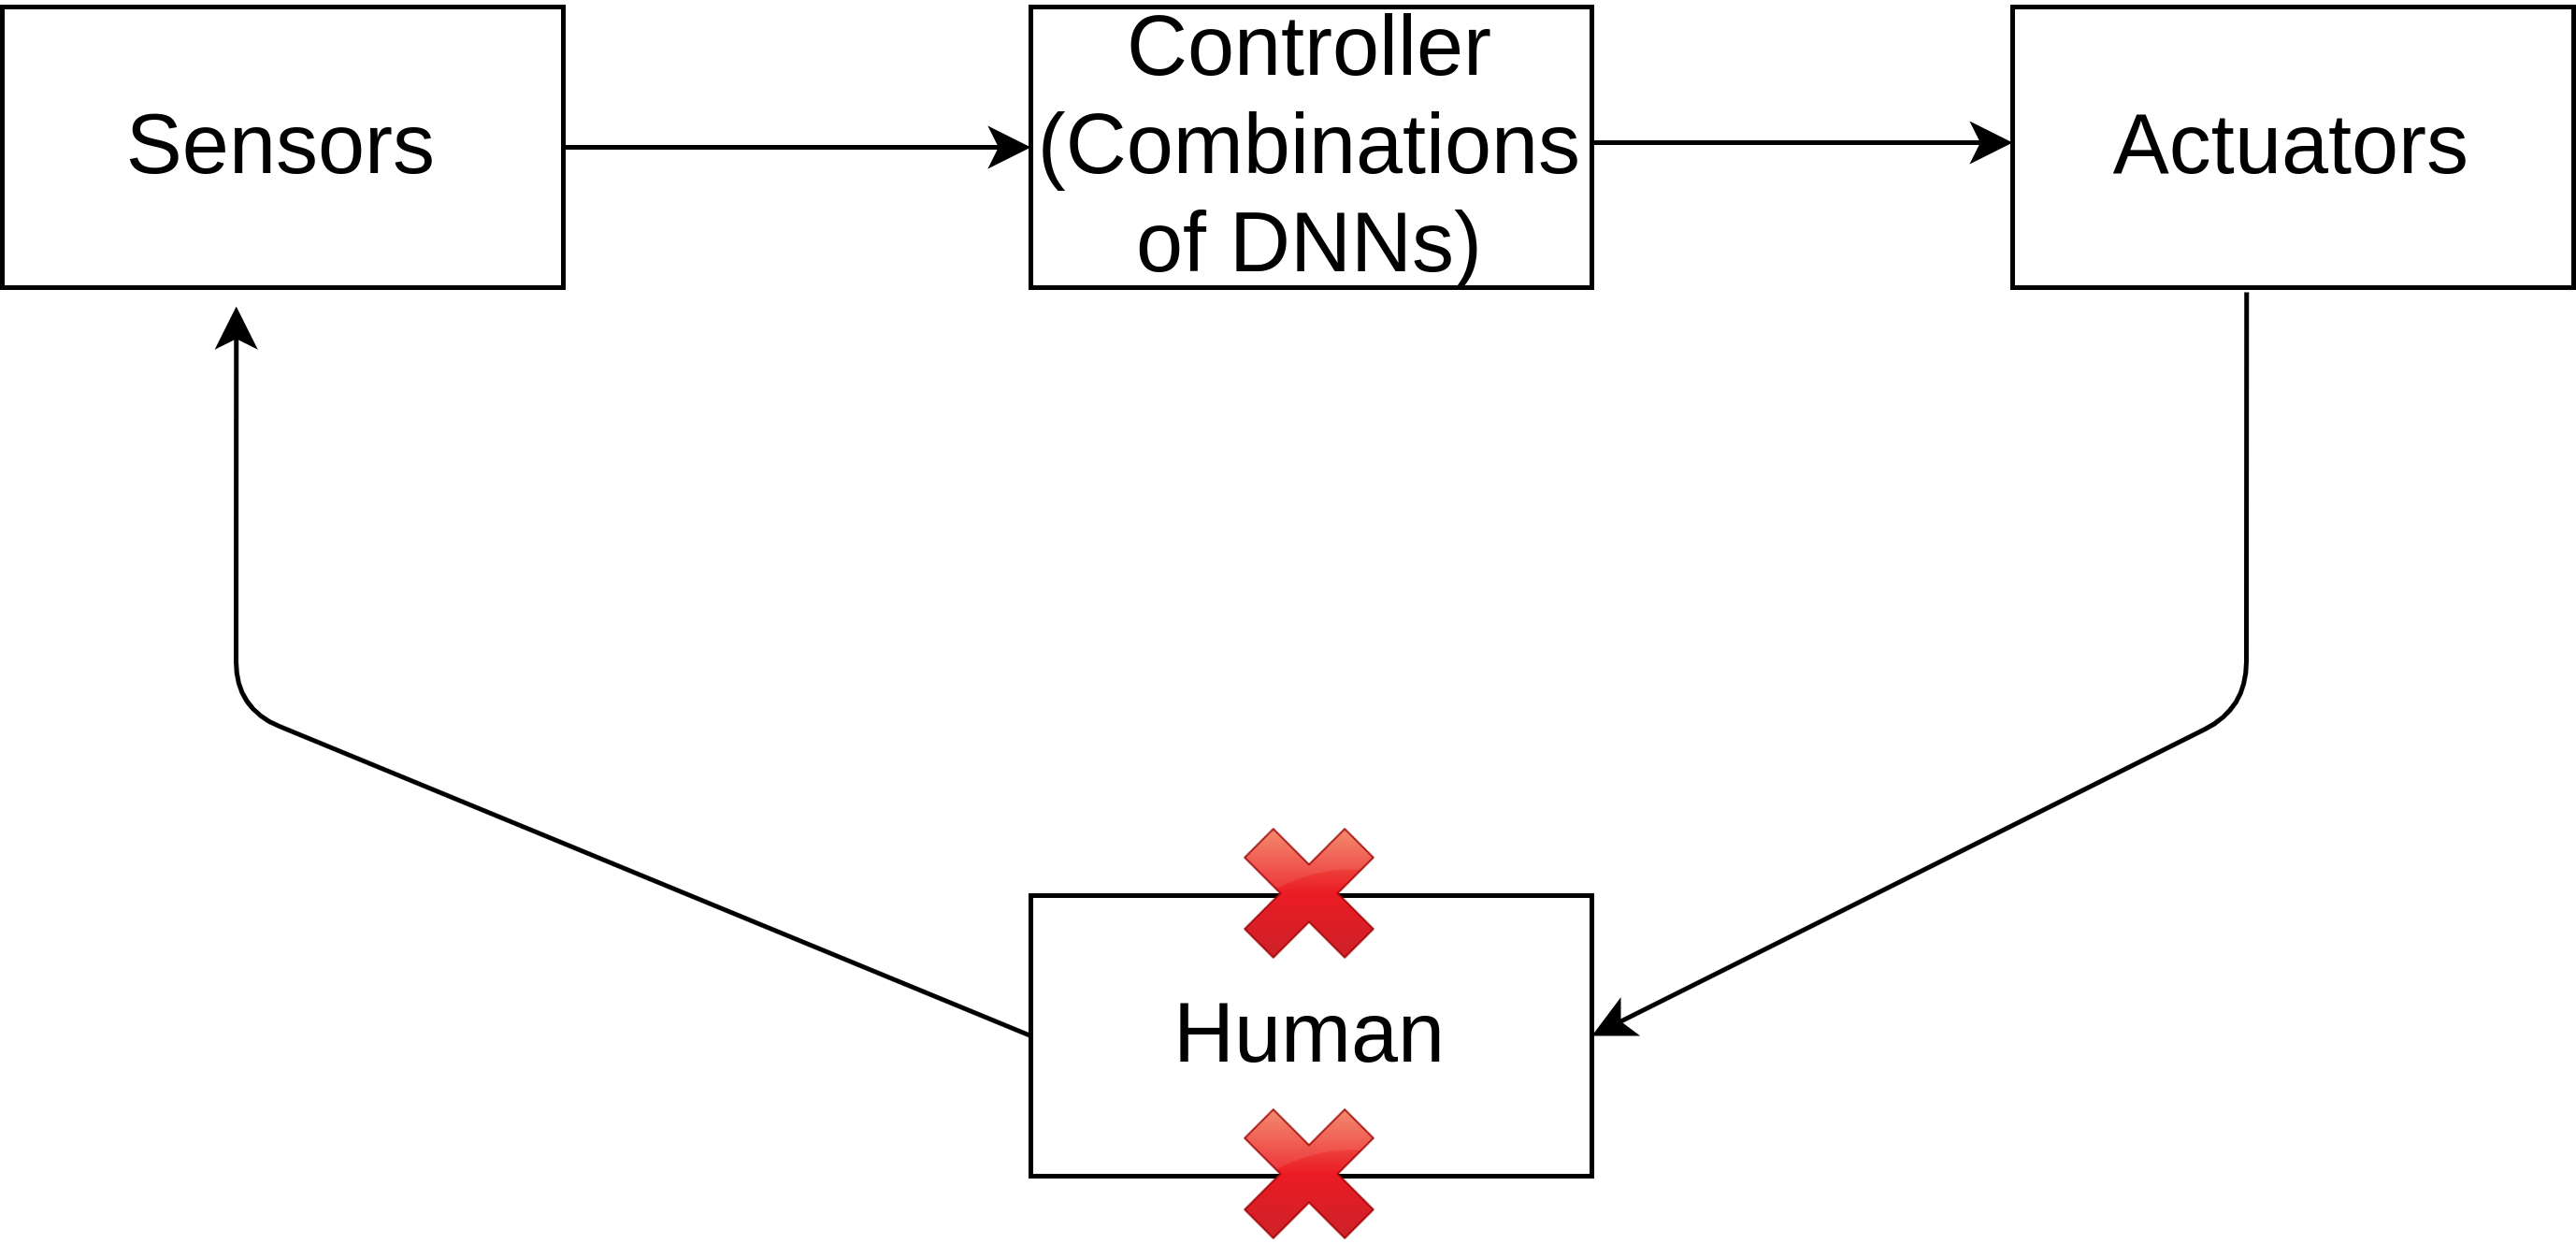
\includegraphics[width=0.7\linewidth]{Images/Systemsdescription}
	\caption[Closed-loop system]{General structure of a closed-loop system without the human involved in the process.}
	\label{fig:systemsdescription}
\end{figure}
\fi

\begin{figure}
	\centering
	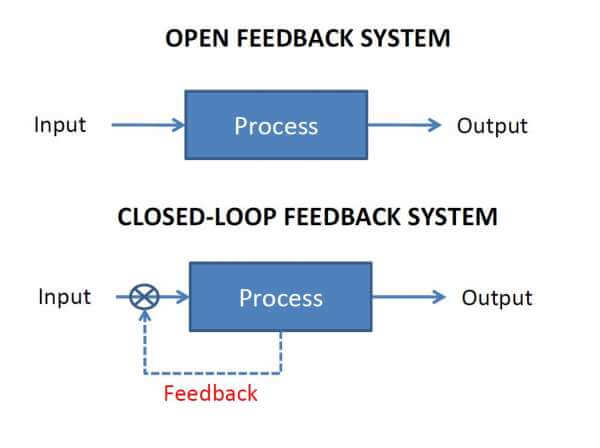
\includegraphics[width=0.7\linewidth]{Images/closedvsopen}
	\caption{General structure of a open and closed-loop systems 
	             Source:https://instrumentationtools.com/open-loop-and-closed-loop-animation/ }
	\label{fig:closedvsopen}
\end{figure}


\section{Cyber-Physical Systems}
\ac{CPS} are systems that combine the cyber part with the physical part that neither could solve alone. CPS based on the data made available make  logical decisions based on the system. For eg. in an insulin pump, the physical data is gathered from the patient which is then used to calculate the  insulin to be injected based on logical formulas and so on the decision making process continues. From Figure 2.1 it can be observed that the decision making process occurs at the controller or the process box where the main logic resides. The data from the physical world is collected from the sensors and the decision making is conducted at the controller and the actuator's job is to physically inject the insulin in the  human which is also the output. 


There are two types of CPS based on the decision making process: open loop and closed loop. In open-loop systems, there is human intervention during the decision making process; as shown in Figure 2.1 the human is a part of the loop where the human keeps a track of the decisions being taken by the controller. 	In closed-loop systems, there are no regular human interventions as shown in Figure 2.1. In the latter case understanding different types of security attacks becomes a necessity. In the case of stealthy (or subtle) attacks as described in the attack model section, the closed loop systems are more vulnerable hence may not raise alarms. The reason is that the existing error-detection mechanisms are not designed to detect small perturbations from the original inputs under a constrained setting that can cause ripples. In DNN based CPS the decision making is accompanied by other DNNs that keep a track of the upper and the lower bounds for error-detection. 

\section{Conventional Controllers for CPS}

%How does a controller work in a conventional setting
A conventional controller takes in the inputs collected through the sensors and processes the input for mode (or state) estimation. There are multiple modes  modeled inside the controller for different scenarios. For eg. in a quadcopter, there are modes for windy flights or normal flights. These modes are important because during a windy weather the flight will have to ensure that the drone is stable and will have to be represented differently as compared to a normal wind flight. Based on the inputs or data collected from the sensors modes are selected. Every mode consists of a different set of equations because every mode represents a different scenario. The outputs are calculated based on the mode that then calculates the next action to be taken by the system. Figure 2.2 shows a position control system of a quadcopter \cite{inbook}. The input values use the derived version of the equations that are used in decision making. 

\begin{figure}
	\centering
	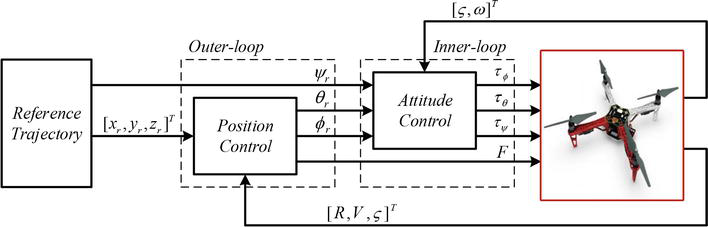
\includegraphics[width=0.7\linewidth]{Images/controltheory}
	\caption{The block diagram of the position control system of the quadcopter.
	}
	\label{fig:controltheory}
\end{figure}


%How are they modeled
These modes are modeled using classical control theory that is represented as a set of equations. These equations are designed by domain experts. For example the model for a medical system such as \ac{APS} can be designed only if the specifications are known for the medical system. A part of the specifications such as the important parameters (insulin, blood glucose etc. in APS) and their threshold values are be provided by domain (in this case medical) experts. Another important aspect for designing control systems is the  modeling precise relations between the parameters. This is possible in systems such as APS because it is a small systems. However, designing the precise mathematical relations for systems such as self-driving cars can be tedious. Therefore, \ac{DNN} have played a huge role in moving the field of autonomous vehicles forward by building models through data. 

  



\section{DNN Based Controller}
The classical controller model is being replaced by DNN based controllers for CPS as shown in  Figure 2.3. The DNN is trained using the data gathered from the traditional control equations. However, during real-time analysis the DNN control is shown to take expert decisions in case of undefined cases. As shown in Figure 2.3 the DNN is the controller and during the training phase the weights and the bias are decided which allows it to control the trajectory in real time. 

One example is the DNN based controller designed by Dutta et al. \cite{Dutta_Others__2018__Robust}. Dutta et al. model robust DNN using available patient data to predict the output in real-time for an insulin pump. Their controller design is for providing a data-driven approach for an artificial pancreas system (APS) which is also our first system for evaluation. 

\begin{figure}
	\centering
	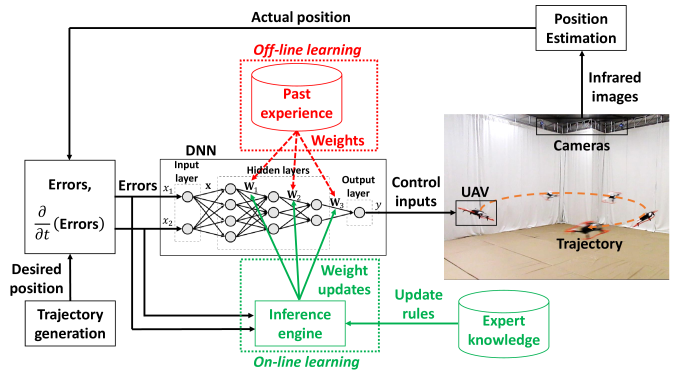
\includegraphics[width=0.7\linewidth]{Images/DNNcontroller}
	\caption{Illustration of how DNN controllers are replacing conventional controllers. The DNN is trained offline using input-output data obtained from different trajectories from a conventional controller. The DNN is shown to perform better than a conventional controller during real-time analysis for decision making.}
	\label{fig:dnncontroller}
\end{figure}

\begin{figure}
	\centering
	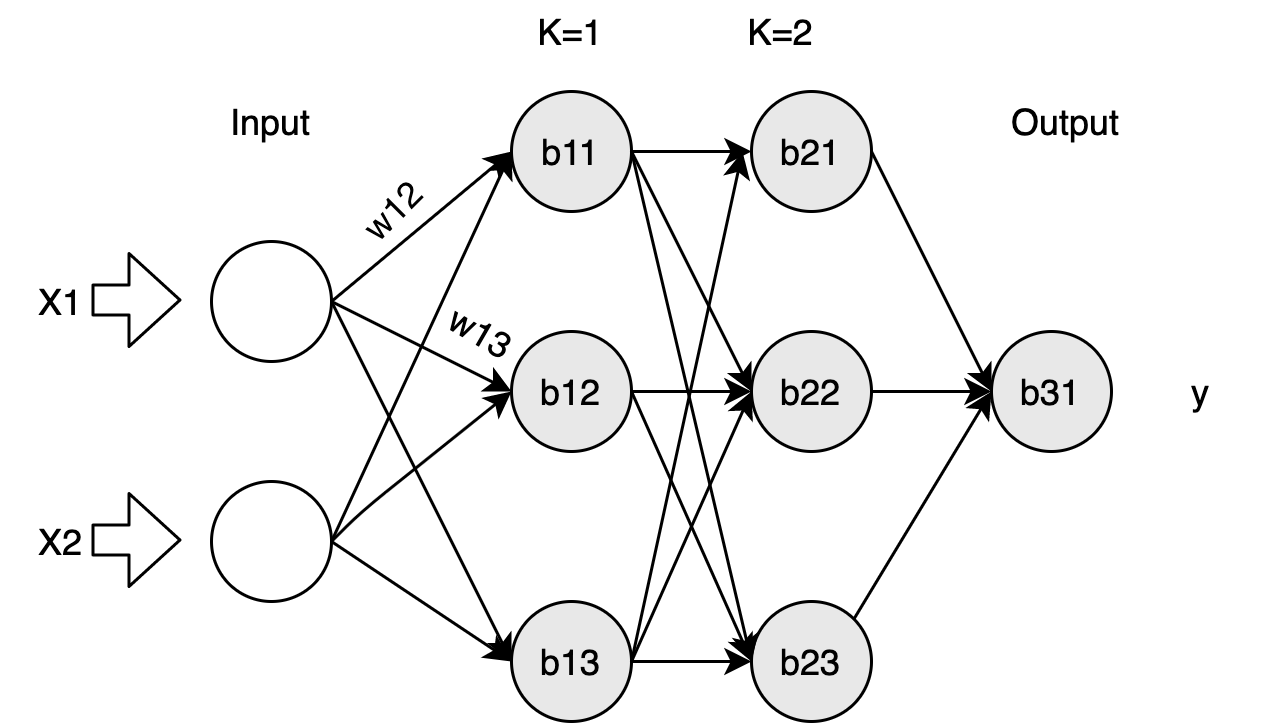
\includegraphics[width=0.7\linewidth]{Images/DNNstructure}
	\caption[DNN structure]{DNN controller structure with two hidden layers K=1,2, two inputs x1 and x2 and one output y. This is an example of a fully connected network.}
	\label{fig:dnn-controller}
\end{figure}

This move towards DNNs over control theory models for modeling \ac{CPS} behaviour can be justified by the following observations: %\ag{you might want to use \textit{itemize/enumerate} to properly format the points. Might become difficult for the reader} 
\begin{enumerate}
	\item CPS behaviour is controlled using a lot of input data from the many sensors a system might have. The self-learning nature of DNNs lends itself well to model behaviour that is driven by the sensor input. This is considered easier than formulating the control theoretic differential equations, which need domain and mathematical expertise \cite{Aamir_2013}.
	To look at a more concrete example, let's turn to a medical system such as \ac{APS}, which uses conventional control theory to build models. Forming the model here requires the programmer to be aware of not only the intended system behaviour, but also the mathematical rigor needed to get the desired result. DNNs, on the other hand, can automatically build models with data.
	Training DNNs is implicitly dependent on the quality of available training data, and it is a known problem in the field \pu{insert refs}. It does not, however, require the system designers to model precise control equations like in control theory.
	\item  There are limitations on the behaviours that can be modelled using the standard control-theoretic approaches. They do not, for instance, work well for building dynamic models \cite{article23}. Building such dynamic models is important in many systems such as in autonomous vehicles, which are essentially composed of multiple interacting control systems. Conventional control systems are not designed to work in an interactive, plug-and-play manner with other control systems because they are built to model only one behaviour. DNNs, by their very nature,  provide this dynamic capability. Due to the data driven modeling using DNNs, it is relatively easier to build models for autonomous vehicles that have multiple models interacting within it. Models for image recognition to detect and lane detection, for instance, can interact continuously with each other to decide the next best course of action.
\end{enumerate}


\section{Roles description}
There are three roles involved in designing and attacking \ac{CPS}.

\begin{enumerate}
	\item \textbf{Specification Designer/Domain Expert:} The domain expert in the realm of \ac{CPS} is responsible for designing the specification documents. For eg. for \ac{APS} the domain expert designs the safe thresholds for the amount of insulin to be injected inside a patient. The domain expert tells values that should trigger alarms in case of a high blood glucose value in a human. 
	
	\item \textbf{System Developer:} These are the people or the designers who based on the specification of the CPS implement the system. For eg. \ac{APS} can be modeled using several different mechanisms. One can use a set of differential equations to design the relations between insulin or blood glucose or one can use \ac{ML} models to build the system models such as decision trees, k-means etc. 
	
	\item \textbf{Attacker:} We are the attackers for the system in the scenario. Our goal is to attack the \ac{CPS} in a stealthy manner. Stealthy here implies we attack the system without getting detected. 
\end{enumerate}
